\begin{ejercicio}\label{ej:50}
  Sea $V_K=\{0,e_1,e_2\}\subset\RR^2$ y $K=\{\{0\},\{e_1\},\{e_2\},\{0,e_1\},\{0,e_2\},\{e_1,e_2\}\}$
  (cf. ejemplo \ref{ejemplo:complejo_circulo}). Prueba que $\abs{K}\approx\Sn^1$, es decir que
  $\Sn^1$ es triangulable.
\end{ejercicio}
%%% RESPUESTA
\begin{proof}%  
  Sabemos que:
  \[
		\abs{K}=\bigcup_{L\in K}\abs{L},
  \]
	pero varios de estos uniendos son redundantes, por ejemplo:
	\[
		\abs{\{v_0\}}=
		\{\sigma\in\abs{K}\,:\, \text{Sop}(\sigma)\subseteq\{v_0\}\subseteq\{v_0,v_1\}\}\subseteq
		\{\sigma\in\abs{K}\,:\, \text{Sop}(\sigma)\subseteq\{v_0,v_1\}\}=
		\abs{\{v_0,v_1\}}.
	\]
	En general la realizaci\'on geom\'etrica de todo 0-simplejo de $K$ est\'a contenido en la realizaci\'on
	geom\'etrica de un 1-simplejo. Por lo tanto:
  \[
		\abs{K}=\abs{\{v_0,v_1\}}\cup\abs{\{v_0,v_2\}}\cup\abs{\{v_1,v_2\}}.
  \]

	Por otro lado, como el conjunto de v\'ertices de $K$ tiene 3 elementos, por definici\'on tenemos que
	$\abs{K}\subset\RR^3$ y cada elemento $\sigma\in\abs{K}$ se escribe como
	$\sigma=(\sigma(v_0),\sigma(v_1),\sigma(v_2))$. De esta manera podemos describir los elementos
	de $\abs{\{v_i,v_j\}}$ como
	\[
		\abs{\{v_0,v_1\}}=
		\{(\sigma(v_0),\sigma(v_1),\sigma(v_2))\in\RR^3\mid 0\leq\sigma(v_i),\,\sigma(v_2)=0,\,\sigma(v_0)+\sigma(v_1)=1\}=
		\{(t,1-t,0)\}_{t\in I}.
	\]
	An\'alogamente:
	\[
		\abs{\{v_0,v_2\}}=	\{(t,0,1-t)\}_{t\in I} \quad\text{y}\quad \abs{\{v_1,v_2\}}=\{(0,t,1-t)\}_{t\in I},
	\]
	y as\'i
	\[
		\abs{K}=\{(t,1-t,0)\}_{t\in I} \cup 	\{(t,0,1-t)\}_{t\in I} \cup \{(0,t,1-t)\}_{t\in I}.
	\]

	Para dar un homeomorfismo entre $\abs{K}$ y $\Sn^1$, dar\'e una composici\'on de tres homeomorfismos:
	\begin{enumerate}
		\item Sea $p:\RR^3\ra\RR^2$ la proyecci\'on $(x,y,z)\mapsto(x,y)$. Claramente $p|_{\abs{K}}$ es continua
			y su imagen es:
			\begin{align*}
				p[\abs{K}]&=
				p\big[\{(t,1-t,0)\}_{t\in I}\big] \cup\, p\big[\{(t,0,1-t)\}_{t\in I}\big] \cup\, p\big[\{(0,t,1-t)\}_{t\in I}\big] \\ &=
				\{(t,1-t)\}_{t\in I} \cup \{(t,0)\}_{t\in I} \cup \{(0,t)\}_{t\in I}.
			\end{align*}
			La funci\'on $p|_{\abs{K}}$ tiene una inversa obvia: para cada pedazo de $p[\abs{K}]$ define
			\begin{eqnarray*}
				q_1:\{(t,1-t)\}_{t\in I} \lra \{(t,1-t,0)\}_{t\in I} &\text{con}& (t,1-t)\mapsto (t,1-t,0) \\
				q_2:\{(t,0)\}_{t\in I} \lra \{(t,0,1-t)\}_{t\in I} &\text{con}& (t,0)\mapsto (t,0,1-t) \\
				q_3:\{(0,t)\}_{t\in I} \lra \{(0,t,1-t)\}_{t\in I} &\text{con}& (0,t)\mapsto (0,t,1-t)
			\end{eqnarray*}
			que son claramente continuas (como restricciones de funciones continuas $\RR^2\ra\RR^3$).
			Adem\'as las podemos pegar porque coinciden en las intersecciones de los dominios:
			\[
				q_1(0,1)=(0,1,0)=q_3(0,1) \;\;,\;\; q_1(1,0)=(1,0,0)=q_2(1,0) \;\;,\;\; q_2(0,0)=(0,0,1)=q_3(0,0).
			\]
			Por lo tanto la funci\'on $q:p[\abs{K}]\ra\abs{K}$, que se obtiene al pegar $q_1,q_2$ y $q_3$ es continua
			y por construcci\'on es la inversa de $p|_{\abs{K}}$. Por lo tanto $p|_{\abs{K}}$ es un homeomorfismo.
			Observa tambi\'en que la imagen de $p|_{\abs{K}}$ es axactamente la frontera de $\Delta^2\subset\RR^2$,
			ie. $p[\abs{K}]=\partial\Delta^2$

		\item Observa que el punto $(1/3,1/3)\in\Delta^2$ est\'a en el interior (porque $1/3+1/3\neq 1$) de $\Delta^2$ ie.
			$(1/3,1/3\not\in\partial\Delta^2)$, entonces aplico la traslaci\'on $(x,y)\mapsto(x-1/3,y-1/3)$ para llevar
			el punto $(1/3,1/3)$ al origen. Esta traslaci\'on es claramente un homeomorfismo. A la traslaci\'on
			de $\partial\Delta^2$ la denoto por $\tau:=\partial\Delta^2-1/3$.

		\item El \'ultimo homeomorfismo es la restricci\'on de normalizar:
			\[
				u:\RR^2\lra\Sn^1 \quad\text{definido por}\quad (x,y)\mapsto\frac{(x,y)}{\sqrt{x^2+y^2}}
			\]
			En coordenadas polares, esta funci\'on hace $(\theta,r)\mapsto(\theta,1)$, entonces s\'olo depende
			del ``argumento'' del vector $(x,y)$.

			Claramente es sobre porque $u|_{\Sn^1}=\Id_{\Sn^1}$. Adem\'as, $u|_{\tau}$ es inyectiva. Para ver
			esto basta observar que cada rayo que inicia en el origen intersecta a $\tau$ en un s\'olo punto, o
			de otra manera: para cada argumento $\theta$ hay un solo vector $(x,y)\in\tau$ con argumento
			igual a $\theta$.

		Por lo tanto $u|_{\tau}:\tau\ra\Sn^1$ es una funci\'on continua y biyectiva. Como $\tau$ es compacto
		(por ser frontera de un 2-simplejo que es compacto) y $\Sn^1$ es Hausdorff, entonces $u|_{\tau}$
		es un homeomorfismo.
	\end{enumerate}

	El siguiente dibujo ilustra los tres pasos:
%
  \begin{figure}[h!]%%%%%%%%%%%%%%%%%%%%%%%%%%%%%%%%%%%%%%%%%%%%%%%%%% FIGURA
    \centering
    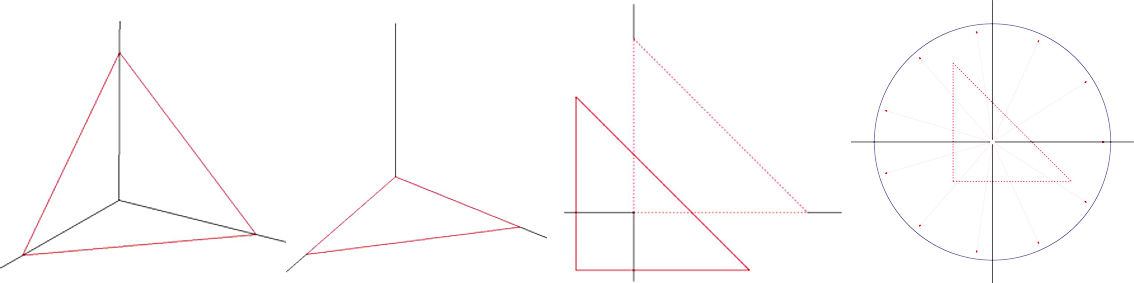
\includegraphics[scale=0.4]{homeomorfismo_circulo}
  \end{figure}%%%%%%%%%%%%%%%%%%%%%%%%%%%%%%%%%%%%%%%%%%%%%%%%%%%%%%%%%%%%%%%%%%%%
%

	Para terminar, simplemente compone los tres homeomorfismos anteriores
	\[
		\abs{K} \lra \partial\Delta^2 \lra \partial\Delta^2-\frac{1}{3} \morf{u} \Sn^1
	\]
	para concluir que $\abs{K}\approx\Sn^1$.











\end{proof}%